\section{Model Documentation}
\begin{multicols}{2}
The section contains the documentation in mathematical form of the underlying age-structured model, and its steady state version that is used to calculate reference points, the observation models used in predicting observations, and the components of the objective function that formulate the statistical criterion (i.e., the objective function) that is used to estimate model parameters.  All of the model equations are laid out in tables and are intended to represent the order of operations, or pseudocode, in which to implement the model.  \iscam\ was implemented in AD Model Builder version 9.0.0 \citep{otterResearch,ADMB2009}.
\end{multicols}

\subsection{Age-structured population model: equilibrium considerations}
\begin{multicols}{2}
For the steady-state conditions represented in Table \ref{Table2}, we assume the parameter vector $\Theta$ in \eqref{T2.1} is unknown and would eventually be estimated by fitting \iscam\ to time series data.  For a given set of growth parameters and maturity-at-age parameters defined by \eqref{T2.3}, growth is assumed to follow von Bertalanffy \eqref{T2.4}, mean weight-at-age is given by the allometric relationship in \eqref{T2.5}, and the age-specific vulnerability is given by a logistic function \eqref{T2.6}.  Note, however, there are alternative selectivity functions implemented in \iscam, the logistic function used here is simply for demonstration purposes.  Mean fecundity-at-age is assumed to be proportional to the mean weight-at-age of mature fish, where maturity at age is specified by the parameters $\dot{a}$ and $\dot{\gamma}$ for the logistic function.

Survivorship for unfished and fished populations is defined by \eqref{T2.8} and \eqref{T2.9}, respectively.  It is assumed that all individuals ages $A$ and older (i.e., the plus group) have the same total mortality rate.  The incidence functions refer to the life-time or per-recruit quantities such as spawning biomass per recruit ($\phi_E$) or vulnerable biomass per recruit ($\phi_b$).  Note that upper and lower case subscripts denote unfished and fished conditions, respectively.  Spawning biomass per recruit is given by \eqref{T2.10}, the vulnerable biomass per recruit is given by \eqref{T2.11} and the per recruit yield to the fishery is given by \eqref{T2.11b}.  Unfished recruitment is given by \eqref{T2.12} and the steady-state equilibrium recruitment  for a given fishing mortality rate $F_e$ is given by \eqref{T2.13}.  Note that in \eqref{T2.13} we assume that recruitment follows a Beverton-Holt model of the form:
\[
R_e=\frac{s_o R_e \phi_e}{1+\beta R_e \phi_e}
\]
where
\[
s_o = \kappa/\phi_E,
\]
\[
\beta = \frac{(\kappa-1)}{R_o\phi_E},
\]
which simplifies to \eqref{T2.13}.
The equilibrium yield for a given fishing mortality rate is \eqref{T2.14}.  These steady-state conditions are critical for determining various reference points such as \fmsy\ and \bmsy.  









%%%%%%%%%%%%%%%%%%%%%%%%%%%%%%%%%%%%%%%%%%%%%%%%%%%%%%%%%%%%%%%%%%%%%%
%%%%%%%%%%%%%%%%%%%%%%%%%%%%%%%%%%%%%%%%%%%%%%%%%%%%%%%%%%%%%%%%%%%%%%
\begin{tablehere}
  %\centering
\caption{Steady-state age-structured model assuming unequal
vulnerability-at-age, age-specific natural mortality, age-specific
fecundity and Beverton-Holt type recruitment.}\label{Table2} 
\tableEq
    \begin{gather}
           \hline
        \mbox{Parameters} \nonumber \\
            \Theta = (B_o,\kappa,M_a,\hat{a},\hat{\gamma}) \label{T2.1}\\
            B_o>0; \kappa > 1; M_a > 0\\
            \Phi = (l_\infty, k, t_o,a,b,\dot{a},\dot{\gamma}) \label{T2.3}\\[1ex]
        %%
        %%
        \mbox{Age-schedule information} \nonumber\\
            l_a=l_\infty(1-\exp(-k(a-t_o)))\label{T2.4}\\
            w_a=a(l_a)^b \label{T2.5}\\
            v_a=(1+\exp(-(\hat{a}-a)/\gamma))^{-1} \label{T2.6}\\
            f_a=w_a(1+\exp(-(\dot{a}-a)/\dot{\gamma}))^{-1} \label{T2.7}\\[1ex]
        %%
        %%
        \mbox{Survivorship} \nonumber\\
            \iota_a=\begin{cases} 1, \quad a=1      \label{T2.8} \\
            \iota_{a-1}e^{-M_{a-1}},\quad a>1\\
            \iota_{a-1}/(1-e^{-M_a}),\quad a=A \end{cases}\\
            \hat{\iota}_a=\begin{cases} 1, \quad a=1\\
            \hat{\iota}_{a-1}e^{-M_{a-1}-F_e v_{a-1}},\quad a>1\\
            \hat{\iota}_{a-1}e^{-M_{a-1}-F_e v_{a-1}}/(1-e^{-M_{a}-F_e v_{a}}),\quad a=A
            \end{cases} \label{T2.9}\\[1ex]
        %%
        %%
        \mbox{Incidence functions} \nonumber \\
            \phi_E=\sum_{a=1}^\infty \iota_a f_a, \quad
            \phi_e=\sum_{a=1}^\infty \hat{\iota}_a f_a \label{T2.10}\\
            \phi_B=\sum_{a=1}^\infty \iota_a w_a v_a, \quad
            \phi_b=\sum_{a=1}^\infty \hat{\iota}_a w_a v_a \label{T2.11}\\
            \phi_q=\sum_{a=1}^\infty
                \frac{ \hat{\iota}_a w_a v_a}{M_a+F_ev_a}
                \left(1-e^{(-M_a-F_ev_a)}\right) \label{T2.11b} \\[1ex]
        %%
        %%
        \mbox{Steady-state conditions} \nonumber \\
        R_o=B_o/ \phi_B \label{T2.12}\\
        R_e=R_o\frac{\kappa-\phi_E/\phi_e}{\kappa-1} \label{T2.13}\\
        %%C_e=R_e \phi_b \frac{F_e}{Z_e}(1-\exp(-Z_e))\label{T2.14} \B \\
        C_e=F_e R_e \phi_q\label{T2.14} \\[1ex]
        \hline \hline \nonumber
    \end{gather}
    \normalEq
\end{tablehere}
%%%%%%%%%%%%%%%%%%%%%%%%%%%%%%%%%%%%%%%%%%%%%%%%%%%%%%%%%%%%%%%%%%%%%%
%%%%%%%%%%%%%%%%%%%%%%%%%%%%%%%%%%%%%%%%%%%%%%%%%%%%%%%%%%%%%%%%%%%%%%

\subsubsection{MSY based reference points}
\iscam\ calculates \fmsy\ based reference points by taking finding the value of $F_e$ that results in the zero derivative of \eqref{T2.14}.  This is accomplished numerically using a Newton-Raphson method where an initial guess for \fmsy\ is set equal to 1.5$M$, then use \eqref{eq1.1} to iteratively find \fmsy.  Note that the partial derivatives in \eqref{eq1.1} can be found in Table \ref{Table3}.

\begin{align}\label{eq1.1}
    F_{e+1}&=F_e - 
    \dfrac{ \dfrac{\partial C_e}{\partial F_e}}
    { \dfrac{\partial^2 C_e}{\partial F_e}}\\
    \mbox{where}\nonumber\\
     \frac{\partial C_e}{\partial F_e} &=
    R_e \phi_q
    + F_e \phi_q \dfrac{\partial R_e}{\partial F_e}
    + F_e R_e \dfrac{\partial \phi_q}{\partial F_e} \nonumber\\
    \frac{\partial^2 C_e}{\partial F_e} &=
    \phi_q \dfrac{\partial R_e}{\partial F_e}
   +  R_e \dfrac{\partial \phi_q}{\partial F_e}\nonumber
%    \frac{R_e \phi_q
%    + F_e \phi_q \dfrac{\partial R_e}{\partial F_e}
%    + F_e R_e \dfrac{\partial \phi_q}{\partial F_e}}
%    {\phi_q \dfrac{\partial R_e}{\partial F_e}
%    +  R_e \dfrac{\partial \phi_q}{\partial F_e}}.
\end{align}

The algorithm usually converges in less than 10 iterations depending on how close the initial guess of \fmsy\ is to the true value.  A maximum of 20 iterations are allowed in \iscam, however, if $\frac{\partial C_e}{\partial F_e}<1e-5$ the algorithm stops.  Note also, that this is only performed on data type variables and not differentiable variables within AD Model Builder.

Given an estimate of \fmsy, other reference points such as MSY are calculated use the equations in Table \ref{Table2} where each of the expressions is evaluated at \fmsy.  A graphical representation of MSY based reference points for two alternative values of the recruitment compensation parameter $\kappa$ is show in Figure \ref{Fig1}.

\begin{figurehere}
  % Requires \usepackage{graphicx}
  \centering
  \psfrag{Re}{$R_e$}
  \psfrag{Fe}{$F_e$}
  \psfrag{Ce}{$C_e$}
  \psfrag{Be}{$B_e$}
  \psfrag{F}{$F_e$}
  \psfrag{SPR}{$\phi_e/\phi_E$}
 %\psfrag{k=12}{$\kappa=12$}
  %\psfrag{k=4}{$\kappa=4$}
  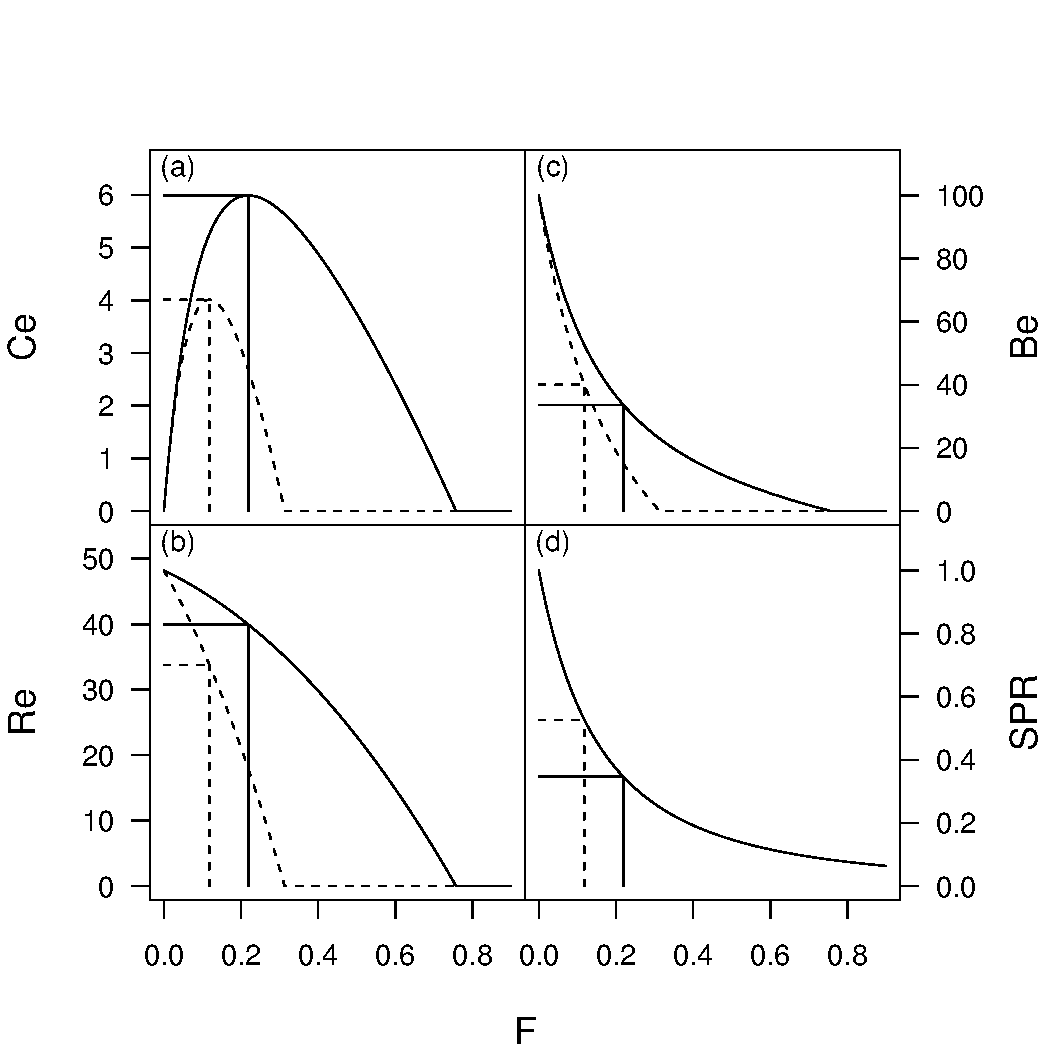
\includegraphics[width=\columnwidth]{iscamFigs/Fig1Quadplot.eps}\\
  \caption{Equilibrium yield (a), recruits (b), biomass (c) and
spawner per recruit ($\phi_e/\phi_E$) (d) versus instantaneous
fishing mortality $F_e$ for two different values of the recruitment
compensation ratio ($\kappa=12$ solid lines, $\kappa=4$ dashed
lines). Vertical lines in each panel correspond to \fmsy\ and
horizontal lines correspond to various reference points that would
achieve MSY.}\label{Fig1}
\end{figurehere}


%%%%%%%%%%%%%%%%%%%%%%%%%%%%%%%%%%%%%%%%%%%%%%%%%%%%%%%%%%%%%%%%%%%%%%
%%%%%%%%%%%%%%%%%%%%%%%%%%%%%%%%%%%%%%%%%%%%%%%%%%%%%%%%%%%%%%%%%%%%%%
\begin{tablehere}
  \centering
\caption{Partial derivatives, based on components in Table
\ref{Table2}, required for the numerical calculation of \fmsy\ using \eqref{eq1.1}.}\label{Table3} \tableEq
    \begin{gather}
        \hline
        \mbox{Mortality \& Survival} \nonumber \\
        Z_{a}=M_a+F_ev_a \label{T3.1} \\
        S_{a}=1-e^{-Z_a}\label{T3.2}\\[1ex]
        %%
        %%
        \mbox{Partial for survivorship} \nonumber \\
        \frac{\partial \hat{\iota}_a}{\partial F_e} =
        \begin{cases}
          0,& a=1 \label{T3.3}\\
          e^{-Z_{a-1}}\left(\dfrac{\partial \hat{\iota}_{a-1}}{\partial F_e}
           -\hat{\iota}_{a-1}v_{a-1}\right),& 1<a<A\\
           \dfrac{\dfrac{\partial \hat{\iota}_{a-1}}{\partial F_e}}
           {1-e^{-Z_a}} -
           \dfrac{\hat{\iota}_{a-1} e^{-Z_{a-1}} v_a e^{-Z_a}}
           {(1-e^{-Z_a})^2}, &a=A
        \end{cases} \\[1ex]
%%        \frac{\partial \hat{\iota}_a}{\partial F_e} =
%%        \begin{cases}
%%          0,& a=1 \label{T3.3}\\
%%          e^{-Z_{a-1}}\left(\dfrac{\partial \hat{\iota}_{a-1}}{\partial F_e}
%%           -\hat{\iota}_{a-1}v_{a-1}\right),& a>1
%%        \end{cases} \\[1ex]
        %%
        %%
        \mbox{Partials for incidence functions} \nonumber \\
        \frac{\partial \phi_e}{\partial F_e}=
            \sum_{a=1}^\infty f_a \frac{\partial \hat{\iota}_a}{\partial
            F_e} \label{T3.4}\\
        %%
        %%
        \frac{\partial \phi_q}{\partial F_e}=
            \sum_{a=1}^\infty \frac{w_av_a S_a}{Z_a}
             \frac{\partial \hat{\iota}_a}{\partial F_e}
             +\frac{\hat{\iota}_a w_av_a^2}{Z_a}\left(e^{-Z_a}-\frac{S_a}{Z_a} \right) \label{T3.5}\\[1ex]
        %%
        %%
        \mbox{Partial for recruitment} \nonumber\\
        \frac{\partial R_e}{\partial F_e}=\frac{R_o}{\kappa-1}
        \frac{\phi_E}{\phi_e^2} \frac{\partial \phi_e}{\partial
        F_e} \label{T3.6}\\[1ex]
        \hline \hline \nonumber
    \end{gather}

    \normalEq
\end{tablehere}
%%%%%%%%%%%%%%%%%%%%%%%%%%%%%%%%%%%%%%%%%%%%%%%%%%%%%%%%%%%%%%%%%%%%%%
%%%%%%%%%%%%%%%%%%%%%%%%%%%%%%%%%%%%%%%%%%%%%%%%%%%%%%%%%%%%%%%%%%%%%%


\end{multicols}



\subsection{Age-structured population model: state-dynamics}
\begin{multicols}{2}
The estimated parameter vector in \iscam\ is defined in \eqref{T4.1}, where $R_0, \kappa$ and $M$ are the leading unknown population parameters that define the overall population scale in the form of unfished recruitment and productivity in the form of recruitment compensation and natural mortality.  The total variance $\vartheta^2$ and the proportion of the total variance that is associated with observation errors $\rho$ are also estimated, then the variance is partitioned into observation errors ($\sigma^2$) and process errors ($\tau^2$) using \eqref{T4.2}.

The unobserved state variables \eqref{T4.3} include the numbers-at-age year year $t$ ($N_{t,a}$), the spawning stock biomass ($B_t$) and the total age-specific total mortality rate ($Z_{t,a}$).

The initial numbers-at-age in the first year \eqref{T4.4} and the annual recruits \eqref{T4.5} are treated as estimated parameters and used to initialize the numbers-at-age matrix.  Age-specific selectivity for gear type $k$ is a function of the selectivity parameters $\gamma_k$ \eqref{T4.6}, and the annual fishing mortality for each gear $k$ in year $t$ ($\digamma_{k,t}$).  The vector of log fishing mortality rate parameters $\digamma_{k,t}$ is a bounded vector with a minimum value of -30 and an upper bound of 3.0.  In arithmetic space this corresponds to a minimum value of 9.36e-14 and a maximum value of 20.01 for annual fishing mortality rates.  In years where there are 0 reported catches for a given fleet, no corresponding fishing mortality rate parameter is estimated and the implicit assumption is there was no fishery in that year.

There is an option to treat natural mortality as a random walk process \eqref{T4.6b}, where the natural mortality rate in the first year is the estimated leading parameter \eqref{T4.1} and in subsequent years the mortality rate deviates from the previous year based on the estimated deviation parameter $\varphi_t$.  If the mortality deviation parameters are not estimated, then $M$ is assumed to be time invariant.

State variables in each year are updated using equations \ref{T4.8}--\ref{T4.11}, where the spawning biomass is the product of the numbers-at-age and the mature biomass-at-age \eqref{T4.8}.  The total mortality rate is given by \eqref{T4.9}, and the total catch (in weight) for each gear is given by \eqref{T4.10} assuming that both natural and fishing mortality occur simultaneously throughout the year.  The numbers-at-age are propagated over time using \eqref{T4.11}, where members of the plus group (age $A$) are all assumed to have the same total mortality rate.  

Recruitment to age $k$ can follow either a Beverton-Holt model \eqref{T4.12} or a Ricker model \eqref{T4.13} where the maximum juvenile survival rate ($s_o$) in either case is defined by $s_o=\kappa/\phi_E$.  For the Beverton-Holt model, $\beta$ is derived by solving \eqref{T4.12} for $\beta$ conditional on estimates of $\kappa$ and $R_o$:
\[
\beta = \frac{\kappa-1}{R_o \phi_E},
\]
and for the Ricker model this is given by:
\[
\beta = \frac{\ln(\kappa)}{R_o \phi_E}
\]

%%%%%%%%%%%%%%%%%%%%%%%%%%%%%%%%%%%%%%%%%%%%%%%%%%%%%%%%%%%%%%%%%%%%%%%%
%%%%%%%%%%%%%%%%%%%%%%%%%%%%%%%%%%%%%%%%%%%%%%%%%%%%%%%%%%%%%%%%%%%%%%%%
\begin{tablehere}
  \centering
\caption{Statistical catch-age model using the Baranov catch
equation and $C^*$ and $F^*$ as leading parameters.}\label{Table4}
\tableEq
    \begin{align}
        \hline \nonumber \\
        &\mbox{Estimated parameters} \nonumber\\
        \begin{split}
        \Theta&= 
        		(R_0,\kappa,M,\bar{R},\rho,\vartheta^2,\gamma_{k},%\bar{F}_k,
        		\digamma_{k,t},\\
		&\quad \{\omega_t\}_{t=1-A}^{t=T},
        		\{\varphi_t \}_{t=2}^T)
	\end{split} \label{T4.1}\\
        \sigma^2&=\rho /\vartheta^2, \quad
        \tau^2=(1-\rho)/\vartheta^2\label{T4.2}\\[1ex]
        %\vartheta^2=\sigma^2+\tau^2, \quad
        %\rho=\frac{\sigma^2}{\sigma^2+\tau^2}\label{T4.3}\\[1ex]
        %%
        %%
        &\mbox{Unobserved states} \nonumber\\
        &N_{t,a},B_t,Z_{t,a}	\label{T4.3}\\
	%%
	%%	        
        &\mbox{Initial states} \nonumber\\
        %v_a=\left[1+e^{-(\hat{a}-a)/\hat{\gamma}}\right]^{-1}\label{T4.7}\\
        N_{t,a}&=\bar{R}e^{\omega_{t-a}} \exp(-M_t)^{(a-1)};\quad t=1;  2\leq a\leq A \label{T4.4}\\
        N_{t,a}&=\bar{R}e^{\omega_{t}} ;\quad 1\leq t\leq T;  a=1 \label{T4.5}\\
        v_{k,a}&=f(\gamma_k) \label{T4.6}\\
        M_t &= M_{t-1} \exp(\varphi_t), \quad t>1 \label{T4.6b}\\
        F_{k,t}&=\exp(\digamma_{k,t}) \label{T4.7}\\[1ex]
        %%
        %%
        &\mbox{State dynamics (t$>$1)} \nonumber\\
        B_t&=\sum_a N_{t,a}f_a \label{T4.8}\\
        Z_{t,a}&=M_t+\sum_k F_{k,t} v_{k,t,a}\label{T4.9}\\
        \hat{C}_{k,t}&=\sum _ a\frac {N_{{t,a}}w_{{a}}F_{k,t} v_{{k,t,a}}
        \left( 1-{e^{-Z_{t,a}}} \right) }{Z_{t,a}}^{\eta_t} \label{T4.10}\\
        %F_{t_{i+1}}= \ F_{t_{i}} -\frac{\hat{C}_t-C_t}{\hat{C}_t'} \label{T4.12}\\
        N_{t,a}&=\begin{cases}
            %\dfrac{s_oE_{t-1}}{1+\beta E_{t-1}} \exp(\omega_t-0.5\tau^2) &a=1\\ \\
            N_{t-1,a-1} \exp(-Z_{t-1,a-1}) &a>1\\
            N_{t-1,a} \exp(-Z_{t-1,a}) & a=A
        \end{cases}\label{T4.11}\\[1ex]
        %%
        %%
        &\mbox{Recruitment models} \nonumber\\
        R_t &= \frac{s_oB_{t-k}}{1+\beta B_{t-k}}e^{\delta_{t}-0.5\tau^2} \quad \mbox{Beverton-Holt} \label{T4.12}\\
        R_t &= s_oB_{t-k}e^{-\beta B_{t-k}+\delta_t-0.5\tau^2} \quad \mbox{Ricker} \label{T4.13}\\
	%%        \mbox{Residuals \& predicted observations} \nonumber\\
	%%        \epsilon_t=\ln\left(\frac{I_t}{B_t}\right)-\frac{1}{n}\sum_{t \in I_t}\ln\left(\frac{I_t}{B_t}\right)\label{T4.15}\\
	%%        \hat{A}_{t,a}=\dfrac{N_{t,a}\dfrac{F_tv_a}{Z_{t,a}}\left(1-e^{-Z_{t,a}}\right)}
	%%        {\sum_a N_{t,a}\dfrac{F_tv_a}{Z_{t,a}}\left(1-e^{-Z_{t,a}}\right)}\label{T4.16}\\
        \hline \hline \nonumber
    \end{align}

    \normalEq
\end{tablehere}
%%%%%%%%%%%%%%%%%%%%%%%%%%%%%%%%%%%%%%%%%%%%%%%%%%%%%%%%%%%%%%%%%%%%%%%%
%%%%%%%%%%%%%%%%%%%%%%%%%%%%%%%%%%%%%%%%%%%%%%%%%%%%%%%%%%%%%%%%%%%%%%%%


\subsubsection{Options for selectivity ($v_{k,t,a}$)} \label{ModelDocSelectivity}

At present, there are six alternative age-specific selectivity options in \iscam.  The simplest of the selectivity options is a simple logistic function with two parameters where it is assumed that selectivity is time-invariant.  The more complex selectivity options assume that selectivity may vary over time a may have as many as (A-1)$\cdot$T parameters.  For time-varying selectivity, cubic and bicubic splines are used to reduce the number of estimated parameters.  Prior to parameter estimation, \iscam\ will determine the exact number of selectivity parameters that need to be estimated based on which selectivity option was chosen for each gear type.  It is not necessary for all gear types to have the same selectivity option.  For example it is possible to have a simple two parameter selectivity curve for say a survey gear, and a much more complicated selectivity option for a commercial fishery.

\paragraph{Logistic selectivity} 
The logistic selectivity option is a two parameter model of the form
\[
v_a = \frac{1}{1+ \exp{(-(a-\mu_{a})/\sigma_a)}}
\]
where $\mu_a$ and $\sigma_a$ are the two estimated parameters representing the age-at-50\% vulnerability and the standard deviation, respectively.

\paragraph{Age-specific selectivity coefficients}
The second option also assumes that selectivity is time-invariant and estimates at total of $A$-1 selectivity coefficients, where the plus group age-class is assumed to have the same selectivity as the previous age-class.  For example, if the ages in the model range from 1 to 15 years, then a total of 14 selectivity parameters are estimated, and age-15+ animals will have the same selectivity as age-14 animals.

When estimating age-specific selectivity coefficients, there are two additional penalties that are added to the objective function that control how much curvature there is and limit how much dome-shaped can occur.  To penalize the curvature, the square of the second differences of the vulnerabilities-at-age are added to the objective function: 
\[
\lambda_k^{(1)} \sum_{a=2}^{A-1}(v_{k,a} - 2v_{k,a-1} + v_{k,a-2})^2
\]
The dome-shaped term penalty as:
\[
\begin{cases}
\lambda_k^{(2)} \sum_{a=1}^{A-1}(v_{k,a} - v_{k,a+1})^2& \mbox(if) v_{k,a+1}< v_{k,a}\\
0 & \mbox(if) v_{k,a+1}\geq v_{k,a}
\end{cases}
\]
For this selectivity option the user must specify the relative weights ($\lambda_k^{(1)},\lambda_k^{(2)}$) to add to these two penalties.

\paragraph{Cubic spline interpolation}
The third option also assumes time-invariant selectivity and estimates a selectivity coefficients for a series age-nodes (or spline points) and uses a natural cubic spline to interpolate between these nodes (Figure \ref{Fig2}). Given $n+1$ distinct knots $x_i$, selectivity can be interpolated in the intervals defined by
\[
S(x) = \begin{cases}
	S_0(x) & x \in [x_0,x_1]\\
	S_1(x) & x \in [x_1,x_2]\\
	...\\
	S_{n-1}(x) & x \in [x_{n-1},x_n]
\end{cases}
\]
where  $S''(x_0) = S''(x_n)=0$  is the condition that defines a natural cubic spline.
\begin{figurehere}
	\centering
	% Requires \usepackage{graphicx}
	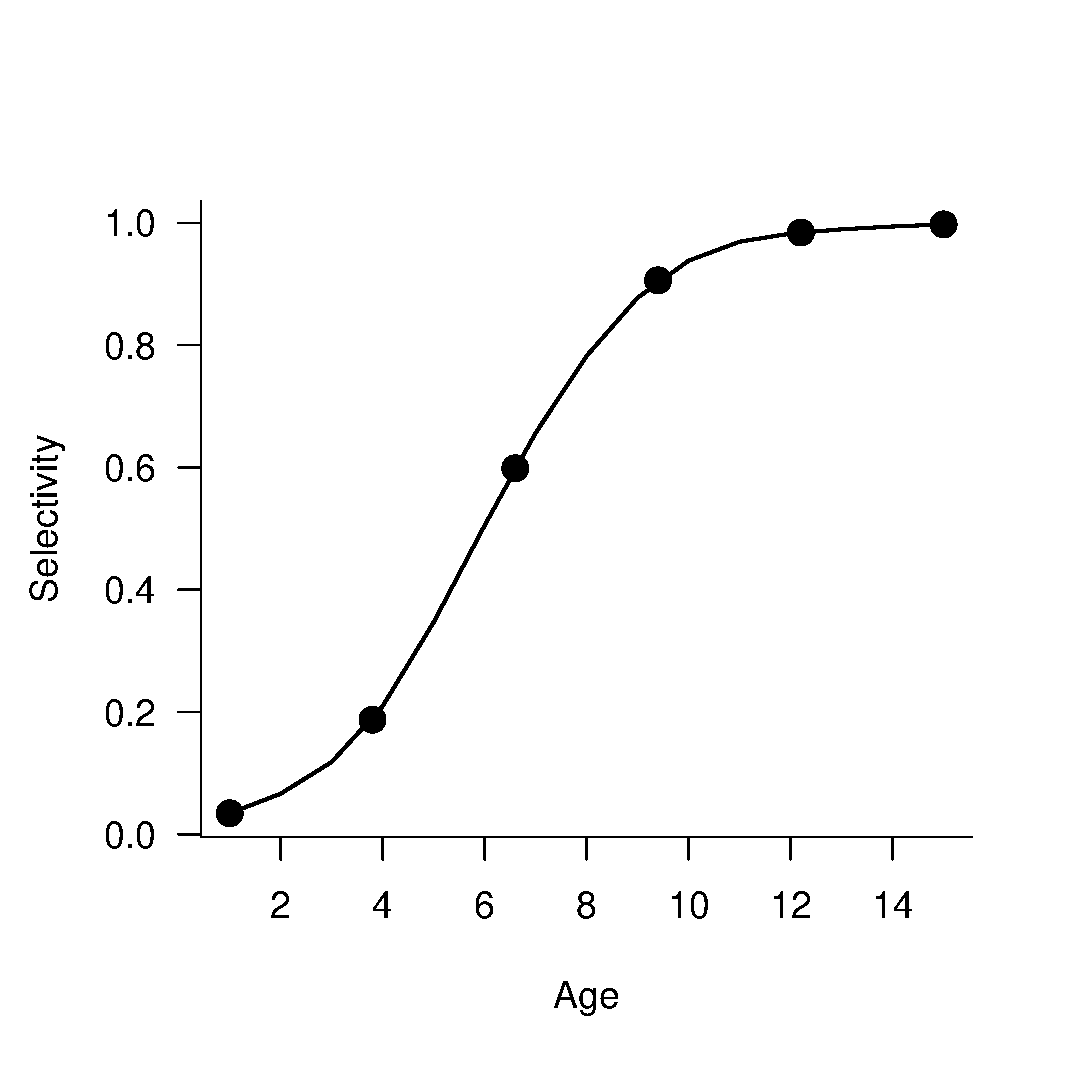
\includegraphics[width=\columnwidth]{iscamFigs/SplineEg.eps}\\
	\caption{Example of a natural cubic spline interpolation for estimating selectivity coefficients.  In \iscam\ the user specifies the number of nodes (circles) to estimate; then age-specific selectivity coefficients are interpolated using a natural cubic spline.}\label{Fig2}
\end{figurehere}

The same penalty functions for curvature and dome-shaped selectivity are also invoked for the cubic spline interpolation of selectivity.

\paragraph{Time-varying selectivity with cubic spline interpolation} A fourth option allows for cubic spline interpolation for age-specific selectivity  in each year.  This option adds a considerable number of estimated parameters but the most extreme flexibility.  For example, given 40 years of data and estimated 5 age nodes, this amounts 200 (40 years times 5 ages) estimated selectivity parameters.  Note that the only constraints at this time are the dome-shaped penalty and the curvature penalty; there is no constraint implemented for say a random walk (first difference) in age-specific selectivity).  As such this option should only be used in cases where age-composition data is available for every year of the assessment.

\paragraph{Bicubic spline to interpolate over time and ages}  The fifth option allows for a two-dimensional interpolation using a bicubic spline (Figure \ref{Fig3}).  In this case the user must specify the number of age and year nodes.  Again the same curvature and dome shaped constraints are implemented.  It is not necessary to have age-composition data each and every year as in the previous case, as the bicubic spline will interpolate between years.  However, it is not advisable to extrapolate selectivity back in time or forward in time where there are no age-composition data unless some additional constraint, such as a random-walk in age-specific selectivity coefficients is implemented (as of \today, this has not been implemented).

\begin{figure*}[!tbp]
	% Requires \usepackage{graphicx}
	\centering
	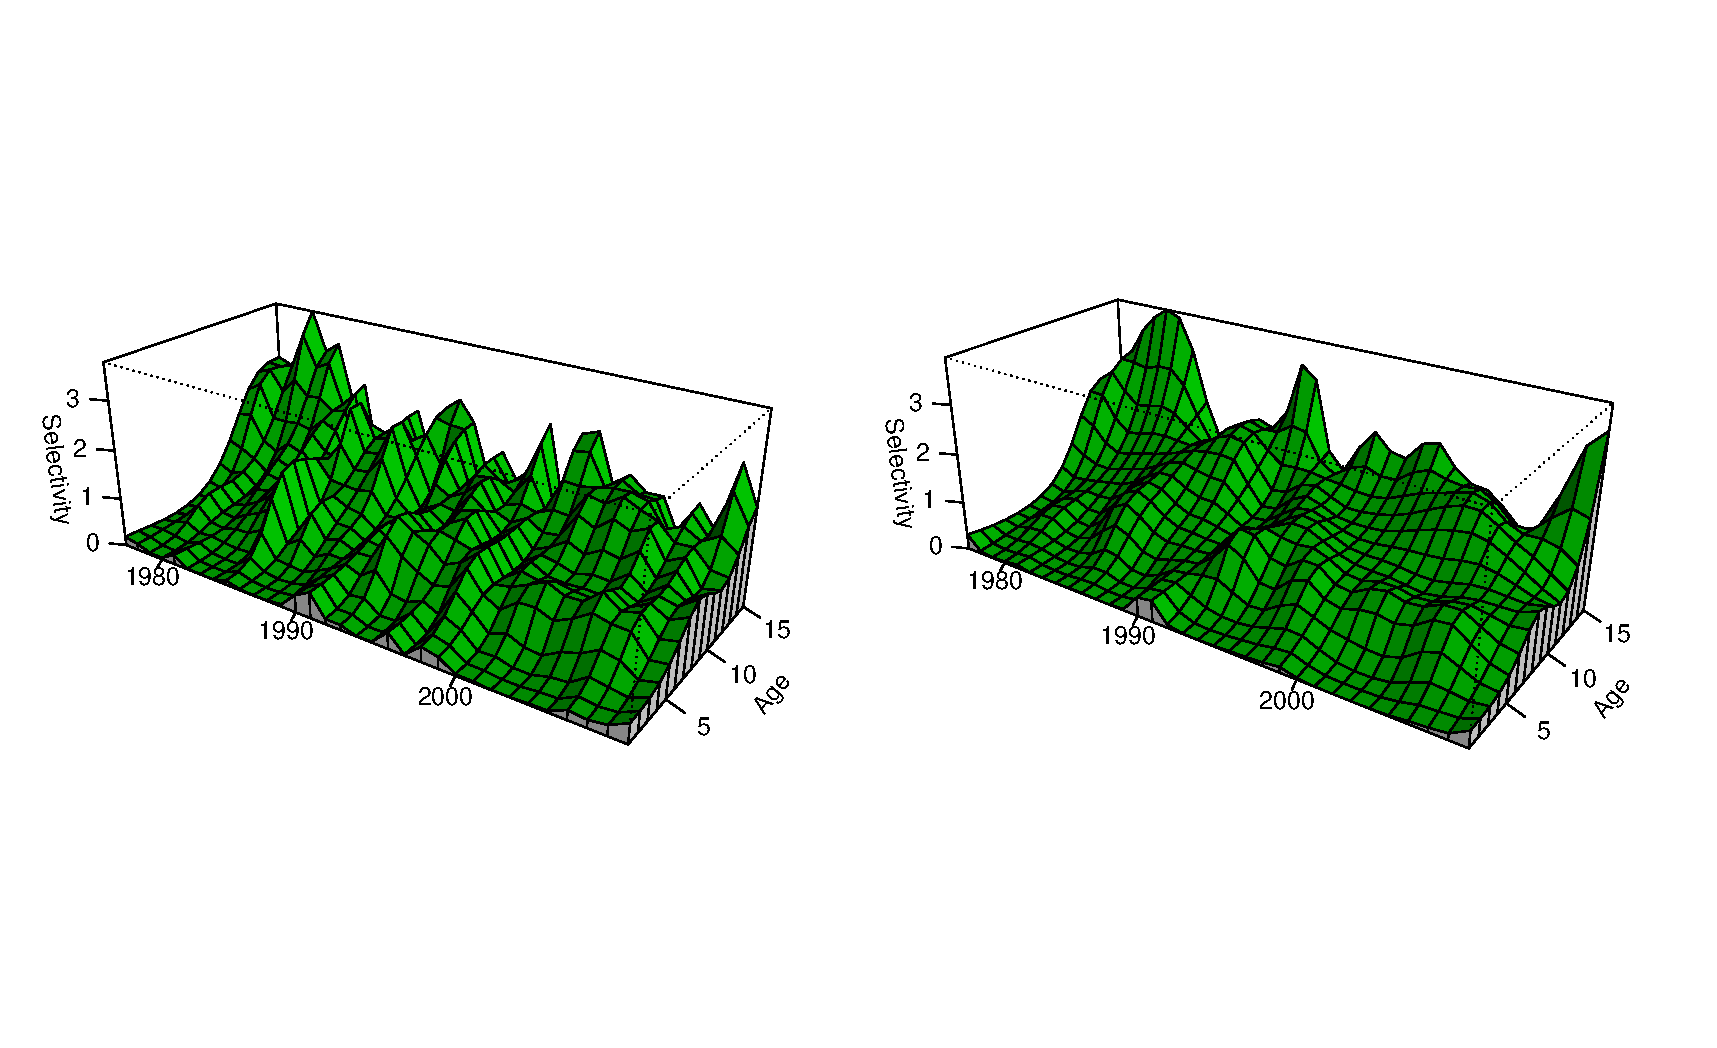
\includegraphics[width=0.9\textwidth]{iscamFigs/BicubicEg.eps}\\
	\caption{Example of a time-varying cubic spline (left) and bicubic spline (right) interpolation for selectivity as applied to the Pacific hake data. The panel on the left contains 165 estimated selectivity parameters and the bicubic interpolation estimates 85 selectivity parameters, or 5 age nodes and 17 year nodes. There are 495 actual nodes being interpolated.}\label{Fig3}
\end{figure*}
\end{multicols}

\subsection{Residuals, likelihoods \& objective function value components}
\begin{multicols}{2}
There are 3 major components to the overall objective function that are minimized while \iscam\ is performing maximum likelihood estimation.  These components consist of the likelihood of the data, prior distributions and penalty functions that are invoked to regularize the solution during intermediate phases of the non-linear parameter estimation.  This section discusses each of these in turn, starting first with the residuals between observed and predicted states followed by the negative loglikelihood that is minimized.

\subsubsection{Catch data}
It is assumed that the measurement errors in the catch observations are log-normally distributed, and the residuals is given by:
\begin{equation}\label{eq2}
\eta_{k,t}=\ln(C_{k,t}+o) -  \ln(\hat{C}_{k,t}+o),
\end{equation}
where $o$ is  a small constant (1.e-10) to ensure the residual is defined in the case of a 0 catch observation.  The residuals are assumed to be normally distributed with a user specified standard deviation $\sigma_{C}$.  At present, it is assumed that observed catches for each gear $k$ is assumed to have the same standard deviation.  To aid in parameter estimation, two separate standard deviations are specified in the control file: the first is the assumed standard deviation used in the first, second, to N-1 phases, and the second is the assumed standard deviation in the last phase.  The negative loglikelihood (ignoring the scaling constant) for the catch data is given by:
\begin{equation}\label{eq3}
\ell_C = \sum_k\left[  T_k\ln(\sigma_C)+\frac{\sum_t(\eta_{k,t})^2}{2\sigma_C^2}\right],
\end{equation}
where $T_k$ is the total number of catch observations for gear type $k$.


\subsubsection{Relative abundance data}
The relative abundance data are assumed to be proportional to biomass that is vulnerable to the sampling gear:
\begin{equation}\label{eq4}
 V_{k,t} = \sum_a N_{t,a} e^{-\lambda_{k,t} Z_{t,a}} v_{k,a} w_a,
\end{equation}
where $v_{k,a}$ is the age-specific selectivity of gear $k$, and $w_a$ is the mean-weight-at-age. A user specified fraction of the total mortality $\lambda_{k,t}$ adjusts the numbers-at-age to correct for survey timing.  The residuals between the observed and predicted relative abundance index is given by:
\begin{equation}\label{eq5}
\epsilon_{k,t} = \ln(I_{k,t}) - \ln(q_k)+\ln(V_{k,t}),
\end{equation}
where $I_{k,t}$ is the observed relative abundance index, $q_k$ is the catchability coefficient for index $k$, and $V_{k,t}$ is the predicted vulnerable biomass at the time of sampling.  The catchability coefficient $q_k$ is evaluated at its conditional maximum likelihood estimate:
\[
  q_k =\frac{1}{N_k} \sum_{t \in I_{k,t}} \ln(I_{k,t}) - \ln(V_{k,t}),
\]
where $N_k$ is the number of relative abundance observations for index $k$ \citep[see][for more information]{walters1994calculation}. The negative loglikelihood for relative abundance data is given by:
\begin{align}
\ell_I &= \sum_k \sum_{t \in I_{k,t}}  \ln(\sigma_{k,t})+\frac{\epsilon_{k,t}^2}{2\sigma_{k,t}^2} \label{eq6}\\
&\mbox{where}\nonumber\\
\sigma_{k,t} &= \frac{\rho \varphi^2}{ \omega_{k,t}},  \nonumber
\end{align}
where $\rho \varphi^2$ is the proportion of the total error that is associated with observation errors, and $\omega_{k,t}$ is a user specified relative weight for observation $t$ from gear $k$.  The $ \omega_{k,t}$ terms allow each observation to be weighted relative to the total error $\rho \varphi^2$; for example, to omit a particular observation, set $\omega_{k,t}=0$, or to give 2 times the weight, then set  $\omega_{k,t}=2.0$. To assume all observations have the same variance then simply set  $\omega_{k,t}=1$.  Note that if  $\omega_{k,t}=0$ then equation \eqref{eq6} is undefined; therefore, \iscam\ adds a small constant to  $\omega_{k,t}$ (1.e-10, which is equivalent to assuming an extremely large variance)  to ensure the likelihood can be evaluated.

\subsubsection{Age composition data}\label{agecomps}
Sampling theory suggest that age composition data are derived from a multinomial distribution \citep{fournier1982general}; however, \iscam\ assumes that age-proportions are obtained from a multivariate logistic distribution \citep{schnute1995influence,richards1997visualizing}.  The main reason \iscam\ departs from the traditional multinomial model has to do with how the age-composition data are weighted in the objective function.  First, the multinomial distribution requires the specification of an effective sample size; this may be done arbitrarily or through iterative re-weighting \citep{MCALLISTER1997,gavaris2002sif}, and in the case of multiple and potentially conflicting age-proportions this procedure may fail to converge properly.  The assumed effective sample size can have a large impact on the overall model results.  

A nice feature of the multivariate logistic distribution is that the age-proportion data can be weighted based on the conditional maximum likelihood estimate of the variance in the age-proportions.  Therefore, the contribution of the age-composition data to the overall objective function is ``self-weighting'' and is conditional on other components in the model.

Ignoring the subscript for gear type for clarity, the observed and predicted proportions-at-age must satisfy the constraint 
\[
 \sum_{a=1}^A p_{t,a} = 1
\]
for each year. The residuals between the observed ($p_{t,a}$) and predicted proportions ($\widehat{p_{t,a}}$) is given by:
\begin{equation}\label{eq7}
\eta_{t,a}=\ln(p_{t,a})-\ln(\widehat{p_{t,a}})-\frac{1}{A}\sum_{a=1}^A\left[\ln(p_{t,a})-\ln(\widehat{p_{t,a}}) \right].
\end{equation}
The conditional maximum likelihood estimate of the variance is given by
\[
\widehat{\tau}^2=\frac{1}{(A-1)T}\sum_{t=1}^T\sum_{a=1}^A \eta_{t,a}^2,
\]
and the negative loglikelihood evaluated at the conditional maximum likelihood estimate of the variance is given by:
\begin{equation}\label{eq8}
	\ell_A = (A-1)T \ln(\widehat{\tau}^2).
\end{equation}
In short, the multivariate logistic likelihood for age-composition data is just the log of the residual variance weighted by the number observations over years and ages.

%Add technical details about requiring the minimum p_{t,a} to be greater than 2% "Grouping".
There is also a technical detail in \eqref{eq7}, where observed and predicted proportions-at-age must be greater than 0.  It is not uncommon in catch-age data sets to observe 0 proportions for older, or young, age classes.  \iscam\ adopts the same approach described by \cite{richards1997visualizing} where the definition of age-classes is altered to require that $p_{t,a}\geq 0.02$ for every age in each year.  This is accomplished by grouping consecutive ages, where $p_{t,a} <0.02$, into a single age-class and reducing the effective number of age-classes in the variance calculation ($\widehat{\tau}^2$) by the number of groups created.  The choice of 2\% is arbitrary and the user can specify the minimum proportion (including 0) to consider when pooling age-proportion data.  In the case of an exact 0 in the observed age-proportions the pooling of the adjacent age-class still occurs, this ensures that \eqref{eq7} is defined.


A \textbf{WARNING} about extremely weak year classes is required here.  A potential problem exists if in fact there is a very small cohort relative to the adjacent cohorts such that it never makes up more than say 2\% (or whatever minimum is specified) of the age-proportions in any given year.  In such cases, the information in the age-composition data about this weak year class relative to of that the adjacent (younger) year class because its always pooled into the younger year class.  \iscam\ will actually estimate two strong cohorts instead of correctly estimating one strong and one weak cohort in the following year.

\subsubsection{Stock-recruitment}
There are two alternative stock-recruitment models available in \iscam: the Beverton-Holt model and the Ricker model.  Annual recruitment and the initial age-composition are treated as latent variables in \iscam, and residuals between estimated recruits and the deterministic stock-recruitment models are used to estimate unfished spawning stock biomass and recruitment compensation.  The residuals between the estimated and predicted recruits is given by
\begin{equation}\label{eq9}
	\delta_t = \ln(\bar{R}e^{w_t}) - f(B_{t-k})
\end{equation}
where $f(B_{t-k})$ is given by either \eqref{T4.12} or \eqref{T4.13}, and $k$ is the age at recruitment.  Note that a bias correction term for the lognormal process  errors is included in  \eqref{T4.12} and \eqref{T4.13}.

The negative log likelihood for the recruitment deviations is given by the normal density (ignoring the scaling constant):
\begin{equation}\label{eq10}
 \ell_\delta = n\ln(\tau) + \frac{\sum_{t=1+k}^T \delta^2_t}{2\tau^2}
\end{equation}
Equations \eqref{eq9} and \eqref{eq10} are key for estimating unfished spawning stock biomass and recruitment compensation via the recruitment models.  The relationship between ($s_o,\beta$) and ($B_o,\kappa$) is defined as:
\begin{align}
s_o &= \kappa/\phi_E\\
\beta&=\begin{cases}
\frac{\kappa-1}{B_o} \quad \mbox{Beverton-Holt}\\[1ex]
\frac{\ln(\kappa)}{B_o} \quad \mbox{Ricker}
\end{cases}
\end{align}
where $s_o$ is the maximum juvenile survival rate, and $\beta$ is the density effect on recruitment.


\end{multicols}

% \clearpage
